\subsection{Encoding a sentence in a vector}
The first aim of this component is encoding a sentence in a vector. The supported internal representation are two:
\begin{itemize}
  % default pooling settings of bert as a service: mean of the second to last layer
  \item \textit{BERT embeddings}. From BERT is even possible to extract embeddings, which have the virtue of being contextual. For this purpose I used ``bert-as-a-service''. For extracting embeddings it uses different pooling strategies: with the default one, does a mean of the vectors of the second-to-last layer. Thus, the dimension of a sentence embedding is $768$, the dimension of a single embedding in BERT Base.
  \item \textit{GloVe embeddings}. GloVe (Global Vectors for Word Representation) is a method of obtaining pre-trained embeddings from a corpus. GloVe is different from and better than its precursor, \textit{word2vec}. This because word2vec takes only local context into account: basically, it considers only words are inside a window span of the sentence.
  
  On the contrary, GloVe tries both to capture meaning in vector space (like word2vec) and to use global count statistics instead of only local information. GloVe learns word embeddings using a co-occurrence matrix, taking in consideration only nonzero elements. The supported dimensions of GloVe embeddings are: 50, 100, 200, 300.
\end{itemize}

In order to find a GloVe representative embedding of a sentence, I did a mean of the vectorized words in the sentence. Obviously, not all the words can be vectorified (some of them might be out-of-vocabulary): for this reason the mean takes in consideration only the vectorized words in the sentence. I tried to limit the number of OOV words importing a large number of GloVe embeddings ($100\,000$). To give a basis for comparison, the current words used in the English language are approximately 171k.

\subsection{Encoding the subsentences of a sentence}
Despite what the reader may expect, this component does not simply encode a sentence in a vector. This because the second aim of this component is to expand the sentence in all its possible sub-sentences (computing the power set of the words in the sentence) and then vectorize them.

The reason behind this choice is that, as we will see in the next section, this procedure provides more flexibility during the mapping of the \textit{tokens for predictions} into symptom concepts.

\begin{figure}[h]
\centering
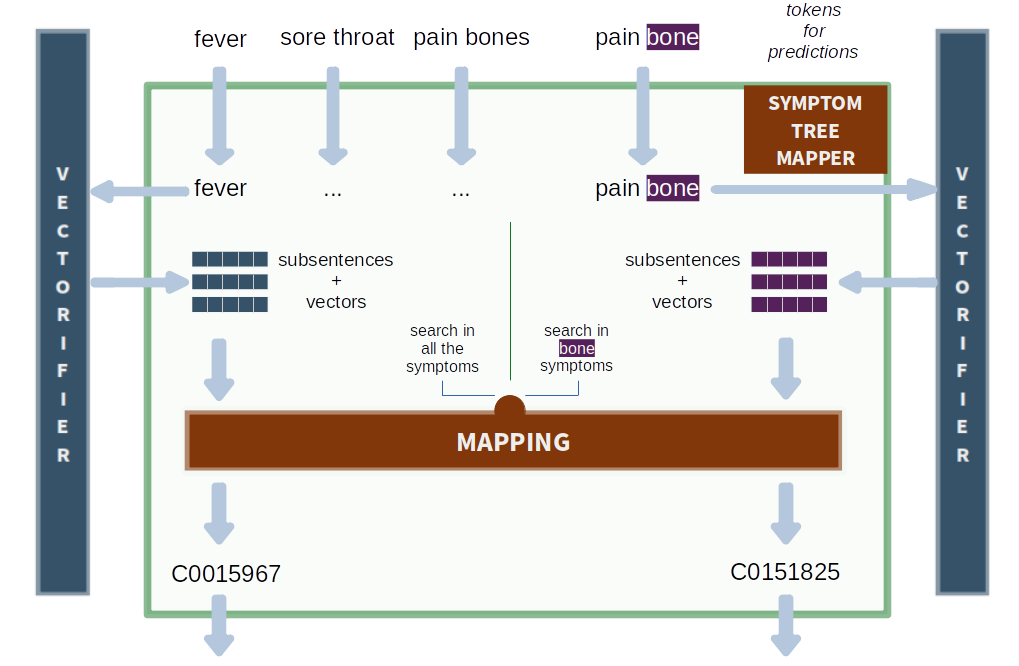
\includegraphics[width=15cm]{symptom_tree_mapper}
\caption{The Symptom Tree Mapper illustrated}
\medskip
\label{fig:symptom_t_m}
\end{figure}
